\documentclass[a4,12pt]{scrartcl}

%Basic 
\usepackage[utf8]{inputenc}
\usepackage[ngerman]{babel}
\usepackage[T1]{fontenc}
%Schrift 
%\usepackage{fontspec} 
%\setmainfont{Arial} 
%Zeilenabstand
\usepackage{setspace}
\setstretch {1.3}
\usepackage{float}
\usepackage[bottom = 3.50cm]{geometry}

%Titel Seite
\usepackage{titling} %Wird benötigt damit \maketitle die Variabeln title, author und date nicht überschreibt
\title{Projektplan}
\subtitle{Projekt: sniffdatel}
\author{David Meister \and Andreas Stalder}		
 %mit /and können Personen hinzugefügt werden
\date{\today}


%Kopf, Fusszeile
\usepackage{fancyhdr}
\pagestyle{fancy}
\lhead{SA Network Unit Testing}
\chead{}
\rhead{netunit}
\lfoot{\thetitle \: v1.0 }
\cfoot{\today }
\rfoot{Seite \thepage}
\renewcommand{\headrulewidth}{0.4pt}

%Bilder
\usepackage{graphicx}

%Zeichnen
\usepackage{tikz}

%Tabellen
\usepackage{booktabs}
\usepackage{longtable}

%Codesnippets
\usepackage{listings}
\lstset{language=java,basicstyle=\footnotesize,frame=single} %backgroundcolor=\color{lightgray}

%Querformat für eine Seite
\usepackage{lscape}
\usepackage{rotating}
\usepackage{pdflscape}

%URL 
\usepackage[colorlinks=true, linkcolor=blue, urlcolor=blue, citecolor=blue]{hyperref}
\urlstyle{same} 


%Loremimpsum
\usepackage{lipsum}



\begin{document}

%\clearpage\maketitle
\begin{titlepage}
	\centering
	\vspace{5cm}
	\begin{center}
%	\includegraphics[width=0.50\textwidth]{}
	\end{center}
	{\huge\bfseries netunit\par}
	\vspace{8cm}
	\raggedright
	{\bfseries SA Network Unit Testing\par}
	{\huge\bfseries Projektplan\par}
	\vspace{1cm}
	{\theauthor \par}
	{\today\par}

\end{titlepage}

\section{Änderungsgeschichte}

\begin{table}[htb]
\centering
    \begin{tabular}{@{} l l l l@{}}\toprule    
    {Datum} & {Version} & {Änderung} & {Autor}\\ \midrule
    27.09.16 & 1.0 & Erstellung erster Version & dm/as\\ \addlinespace
    \end{tabular}
\caption{\textbf{Änderungsgeschichte}}
\end{table}

\newpage

%\thispagestyle{empty}
\tableofcontents
\newpage


\section{Einführung}
\subsection{Zweck}
Dieses Dokument stellt den Projektplan für unser Studienarbeit dar, es dient zur Planung, Steuerung und Kontrolle.
\subsection{Gültigkeitsbereich}
Dieses Dokument ist über die gesamte Projektdauer gültig. Es wird in späteren Iterationen angepasst. Somit ist jeweils die neuste Version des Dokuments gültig und alte Versionen sind obsolet.
\subsection{Referenzen}
\begin{description}
Noch keine.
%  \item[jNetPcap] \hfill \\
%  \url{http://jnetpcap.com/}
\end{description}

\section{Projekt Übersicht}

\subsection{Zweck und Ziel}

\subsection{Lieferumfang}

\subsection{Annahmen und Einschränkungen}

\subsection{Organisationsstruktur}
\begin{table}[H]
\centering
    \begin{tabular}{@{} l l l l@{}}    
    {Vorname} & {Name} & {E-Mail} & Veratwortlich für\\ \midrule
    Andreas & Stalder & astalder@hsr.ch & -\\ \addlinespace
    David & Meister & dmeister@hsr.ch & -\\ \bottomrule
    \end{tabular}
\caption{\textbf{Teammitglieder}}
\end{table} 

\subsection{Externe Schnittstellen}
Das Projekt wird von Beat Stettler und Urs Baumann betreut und benotet.

\section{Management Abläufe}
\subsection{Kostenvoranschlag}
Der Projektstart ist am Montag den 22. September 2016. \\
Die Projektdauer beträgt 14 Wochen, und das Projektende ist am Freitag den 23. Dezember 2016. \\


\noindent Während diesen 14 Wochen sind 240 Arbeitsstuden pro Projektmitglied eingeplant. Das entspricht pro Mitglied eine Arbeitszeit von 18 Stunden pro Woche. Dies ergibt einen totalen Aufwand von 480 Stunden.\\

\noindent Die wöchentliche Arbeitszeit von 18 Stunden kann bei Verzug oder bei unerwarteten Problemen auf maximal 24 Stunden erhöht werden. \\

\noindent Es sind gegenwärtig keine Absenzen während dieser Zeit geplant. 
\subsection{Zeitliche Planung}
Die Zeitplanung und die Verwaltung der Arbeitspakete erfolgt in Redmine. Diese wird während dem Projekt laufend aktualisiert. Die im Redmine erzeugten Tickets dienen als Arbeitspakete. Diese werden einer, ebenfalls im Redmine hinterlegten, Iteration zugewiesen. Anhand von diesen Daten ist ein übersichtlicher Zeitplan ersichtlich. Um einen Überblick über den aktuellen Zeitplan zu erhalten, erfolgt der Zugriff auf das Gantt-Diagram via URL:
Die Projektmitglieder tragen jeweils die investierte Zeit am Abend, in das zugewiesene Ticket ein. 

\subsubsection{Phasen}
Das Projekt wird in fünf Phasen unterteilt: Initialisierung, Analyse, Design, Construction und Abschluss.
\newline
\newline
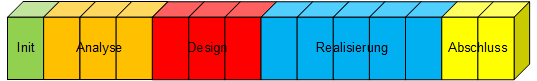
\includegraphics[width=1\textwidth]{figures/phasen.png}
\newpage

\subsubsection{Meilensteine}
Das Projekt beinhaltet insgesamt fünf Meilensteine. \\
\begin{table}[H]
    \begin{tabular}{@{} l l l r@{}}\toprule    
    {Meilenstein} & {Beschreibung} & {Datum}\\ \midrule
    MS1 & Anforderungen und Scope definiert  & 13.10.16\\ \addlinespace
    MS2 & Architektur und Design beschrieben & 27.10.16\\ \addlinespace
    MS3 & Betaversion fertiggestellt  & 17.11.16\\ \addlinespace
    MS4 & Software und Dokumentationen fertiggestellt  & 08.12.16\\ \addlinespace
    MS5 & Arbeitsabgabe & 23.12.16\\ 
    \bottomrule
    \end{tabular}
\caption{\textbf{Projekt Meilensteine}}
\end{table}


\subsubsection{Iterationen}
Die Dauer eines Iterationszyklus beträgt jeweils eine Wochen. 
\begin{table}[htb]
\centering
    \begin{tabular}{@{} p{3cm} l l l@{}}\toprule    
    {Iteration} & {Inhalt} & {Start} & {Ende}\\ \midrule
    Initialisierung & Projektstart und Kickoff-Meeting & 15.09.2016  & 22.09.2016\\ \addlinespace
    Analyse 1 & Projektplanung  & 23.09.2016 & 30.09.2016\\ \addlinespace
    Analyse 2 & -  & 01.10.2016 & 06.10.2016\\ \addlinespace
    Analyse 3 & -  & 07.10.2016 & 13.10.2016\\ \addlinespace
    Design 1 & - & 14.10.2016 & 20.10.2016\\ \addlinespace
    Design 2 & - & 21.10.2016 & 27.10.2016\\ \addlinespace
    Realisierung 1 & - & 28.10.2016  & 03.11.2016\\ \addlinespace
    Realisierung 2 & - & 04.11.2016  & 10.11.2016\\ \addlinespace
    Realisierung 3 & - & 11.11.2016  & 17.11.2016\\ \addlinespace
    Realisierung 4 & - & 18.11.2016  & 24.11.2016\\ \addlinespace
    Realisierung 5 & - & 25.11.2016  & 01.12.2016\\ \addlinespace
    Realisierung 6 & - & 02.12.2016  & 08.12.2016\\ \addlinespace
    Abschluss 1 & - &  09.12.2016 & 15.12.2016\\ \addlinespace
    Abschluss 2 & - &  16.12.2016 & 23.12.2016\\ \addlinespace
    \bottomrule
    \end{tabular}
\caption{\textbf{Projekt Iterationen}}
\end{table}


\begin{landscape}
\subsubsection{Arbeitspakete (Tickets)}
\begin{longtable}{ p{5.5cm} p{8cm} l l p{1cm} p{1cm} }

\hline 
\multicolumn{1}{p{5.5cm}}{\textbf{Name}} & \multicolumn{1}{p{8cm}}{\textbf{Inhalt}} & \multicolumn{1}{l}{\textbf{Iteration}} & \multicolumn{1}{l}{\textbf{Wer}} & \multicolumn{1}{p{1cm}}{\textbf{Soll}} & \multicolumn{1}{p{1cm}}{\textbf{Ist}} \\ \hline 
\endfirsthead


\hline 
\multicolumn{1}{p{5.5cm}}{\textbf{Name}} & \multicolumn{1}{p{8cm}}{\textbf{Inhalt}} & \multicolumn{1}{l}{\textbf{Iteration}} & \multicolumn{1}{l}{\textbf{Wer}} & \multicolumn{1}{p{1cm}}{\textbf{Soll}} & \multicolumn{1}{p{1cm}}{\textbf{Ist}} \\ \hline 
\endhead


\textbf{Projektstart}&&&&\\ \addlinespace
Kickoff-Meeting & Allgemeine Besprechungen zum Projektstart & Initialisierung & Alle & 1 & 0.75 \\ \addlinespace
\hline\caption{\textbf{Arbeitspakete}}
\end{longtable}
\end{landscape}




\subsection{Teammeeting}
Besprechungen finden wöchentlich jeweils am Dienstag statt. 
Eine Besprechung dauert in der Regel 30min und findet in der HSR statt. Bei einer Besprechung wird das weitere Vorgehen, sowie durchgeführte Arbeiten, fällige Arbeiten und auftretende Probleme besprochen. Weiter werden Arbeitspakete verteilt, damit beide Projektmitglieder wissen was zu tun ist. 

\subsubsection{Meeting mit Betreuern}
Die Meetings mit den Betreuern finden jeden Donnerstag um 13:30 Uhr statt. 
Die Meetings werden mit den Betreuern Beat Stettler und Urs Baumann in ihrem Büro durchgeführt. Die Dauer eines Meetings ist unterschiedlich und kann stark variieren. 

\section{Risikomanagement}
\subsection{Risiken}
Technische Risiken in der Entwicklung sind im Dokument TechnischeRisiken.xlsx aufgeführt.
\subsection{Umgang mit Risiken}
Die im Dokument TechnischeRisiken.xlsx aufgeführten Risiken sind in der Zeitplanung nicht speziell vorgesehen. Falls beim Eintreten eines geplanten Risikos ein erhöhter Zeitbedarf entsteht, so muss dies mit hoher Wahrscheinlichkeit mit Mehrarbeit der Teammitglieder kompensiert werden. Falls die nötige Mehrarbeit ausserhalb der Möglichkeiten liegt, so muss in Absprache aller Teammitglieder mit dem Betreuer nach einer anderer Lösung (z.B. Einschränkung von Programmfeatures, etc.) gesucht werden.


\section{Qualitätsmassnahmen}

\begin{table}[H]
\centering
    \begin{tabular}{@{} p{3cm} p{4cm} p{6cm} @{}}\toprule    
    {Massnamen} & {Zeitraum} & {Ziel der Massnahme}\\ \midrule
    Git verwenden & immer & Versionierung und Verhinderung von Datenchaos\\ \addlinespace
    Redmine verwenden & immer & Einhaltung von Vorgehen und Zeitplan\\ \addlinespace
    Teamsitzung & 1h pro Woche & Sicherstellung der erfolgreichen Kommunikation.\\ \addlinespace
    Codereviews & nach Abschluss von Ticket & Garantierung guter Codequalität  \\ \addlinespace
    Styleguide für Code & immer & Code lesbarkeit und Wartungsfreundlichkeit\\ \addlinespace
    Tests & in und nach der Programmierphase & Sicherstellung der Funktionalität \\
    \bottomrule
    \end{tabular}
\caption{\textbf{Qualitätsmassnahmen}}
\end{table}

\subsection{Dokumentation}
Alle Datein, welche Teil der Dokumentation sind, werden mit Git versioniert. Das Git Repository befindet sich auf GitHub.
\subsection{Projektmanagement}
Als Projektmanagementsoftware wird Redmine eingesetzt. 
Es wird nach jeder Arbeitssession oder beim Wechsel einer Arbeit der Aufwand auf das entsprechende Ticket verbucht.
Zugriff auf Redmine erfolg über die Url: - % TODO: noch erfassen}
Um den Zugriff für Betreuungspersonen zu ermöglichen wurde ein Gastbenutzer eingerichtet.
\newline
\newline
Logindaten Redmine Gastbenutzer:
\begin{description}
\begin{description}
\item [Login:]
-
% TODO: Login erfassen
\item [Password:]
-
% TODO: Login erfassen
\end{description}
\end{description}


\subsection{Entwicklung}
Wie die Dokumentation wird auch der Code mit Git versioniert und auf GitHub abgelegt.

\subsubsection{Vorgehen}
Als Erstes erfolgt die Einarbeitung in das entsprechende Thema.
Nach Erstellung eines Konzeptes werden die Features separiert entwickelt.
Wurden Reviews und Tests erfolgreich durchgeführt, kann die Zusammenführung erfolgen.


\subsubsection{Code Reviews}
Damit wir eine Kontrolle über den Code haben, wird jedes Feature von mindestens einer anderen Person betrachtet.
Dazu wird wie folgt vorgegangen: \\
Die zuständige Person entwickelt das vorgesehene Feature und schreibt Tests dazu.
Wenn man mit seiner Arbeit zufrieden ist, bekommt das Feature den Status Feedback.
All diese Feedback-Tickets werden einmal pro Woche von mindestens einem anderen Teammitglied überprüft.
Wenn alles in Ordnung ist, wird das Ticket auf Erledigt gesetzt.
Falls ein Fehler gefunden wurde, wird ein Kommentar hinzugefügt und das Ticket bekommt den Status In Bearbeitung.



\end{document}

